\documentclass{standalone}
\usepackage{tikz}
\usepackage{ctex,siunitx}
\usepackage{tkz-euclide}
\usepackage{amsmath}
\usetikzlibrary{patterns, calc}
\usetikzlibrary {decorations.pathmorphing, decorations.pathreplacing, decorations.shapes,}
\begin{document}
\small
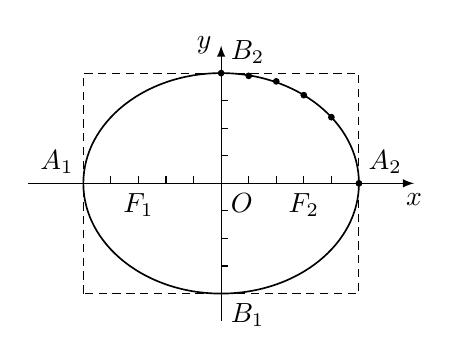
\begin{tikzpicture}[>=latex,scale=0.35]
  \draw[thin,->](-7,0)--(7,0)node[below]{$x$};
  \draw[thin,->](0,-5)--(0,5)node[left]{$y$};
  \draw[semithick](0,0)ellipse(5 and 4);
  \tkzDefPoints{0/0/O,-3/0/F1,3/0/F2,0/4/A,1/3.9/B,2/3.7/C,3/3.2/D,4/2.4/E,5/0/F}
  \draw[densely dashed](-5,-4)rectangle(5,4);
  \foreach \x in {1,2,3,-1,-2,-3}
    {
      \draw[thin](\x,0)--++(0,0.25);
      \draw[thin](0,\x)--++(0.25,0);
    }
  \draw[thin](-4,0)--++(0,0.25)(4,0)--++(0,0.25);
  \tkzDrawPoints[fill=black](A,B,C,D,E,F)
  \tkzLabelPoint[below](F1){$F_1$}
  \tkzLabelPoint[below](F2){$F_2$}
  \tkzLabelPoints[below right](O)
  \node at (-5,0)[above left]{$A_1$};
  \node at (5,0)[above right]{$A_2$};
  \node at (0,-4)[below right]{$B_1$};
  \node at (0,4)[above right]{$B_2$};
\end{tikzpicture}
\end{document}